\chapter{Lecture}\label{part1:lec4}
\markboth{\thechapter. Lecture}{\thechapter. Lecture}

In\pageoriginale  the last lecture we proved the surprising theorem on pentagonal
numbers:
\begin{equation*}
  \prod^\infty_{m=1} (1- x^m) = \sum^\infty_{\lambda=-\infty}
  (-)^\lambda x^{\lambda (3 \lambda-1)/2} \tag{1}\label{part1:lec4:eq1}
\end{equation*}

We do not need these identities for their own sake, but for their
applications to number theory. We have the same sort of power-series
on both sides; let us compare the coefficients of $x^n$. On the left
side $n$ appears as the sum of different exponents. But in
contradiction to previous situations, the coefficients appear with
both positive and negative signs, so that when we collect the terms
there may be cancellations. There are gaps in the powers that appear,
but among those which appear with non-zero coefficients, we have a
pair of positive terms followed by a pair of negative terms and vice
versa. In most cases the coefficients are zero; this is because of
cancellations, so that roughly terms with positive and negative signs
are in equal number. A positive  sign appears if we multiply an even
number of times. otherwise a negative sign. So an even number of
different summands is as frequent generally as an odd number. Hence
the following theorem:

The number of decompositions of $n$ into an even number of different
parts is the same as the number of decompositions into an odd number,
with the exception that there is a surplus of one sort or the other if
$n$ is a pentagonal number of the form $\lambda (3 \lambda-1)/2$.

Before proceeding further let us examine a number of concrete
instances. Take 6 which is not a pentagonal number. The partitions are\pageoriginale 
6, $1+5$, $2+4$, $1+2+3$, so that there are two decompositions into an
even number of different parts, and two into an odd number. Next take
7, which is a pentagonal number, $7= \frac{\lambda(3 \lambda+1)}{2}$
with $\lambda=2$. We can actually foresee that the excess will be in
the even partitions. The partitions are 7, $1+6$, $2+5$, $3+4$,
$1+2+4$. Take 8 which again is not pentagonal. We have three in each
category: 8, $1+7$, $2+6$, $3+5$, $1+2+5$, $1+3+4$.

This is a very extraordinary property of pentagonal numbers. One would
like to have a direct proof of this. A proof is due to Fabian Franklin
(Comptes Rendus, Paris. 1880), a pupil of the famous Sylvester. The
proof is combinatorial. We want to establish a one-one correspondence
between partitions containing an even number of summands and those
containing an odd number - except for pentagonal numbers.

Consider a partition with the summands arranged in increasing order,
each summand being denoted by a horizontal row of dots. Mark
specifically the first row,

\begin{figure}[H]
  \centering{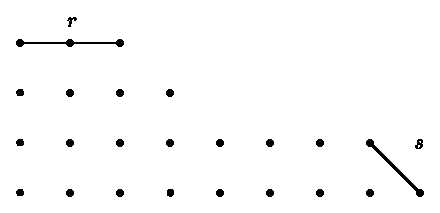
\includegraphics{vol2-figures/fig2.7.eps}}
\end{figure}
with $r$ dots, and the last slope, with $s$ dots i.e., points on or
below a segment starting from the dot on the extreme right of the
last row and inclined at $45^\circ$ (as in the diagram). We make out
two cases. 
\begin{enumerate}
\item $s < r$. Transfer the last slope to a position immediately above
  the first row. The diagram is now as shown below:
  \begin{figure}[H]
    \centering{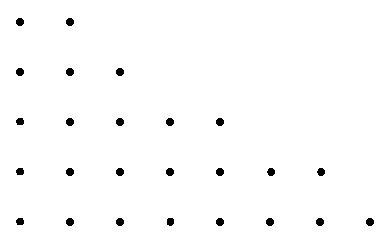
\includegraphics{vol2-figures/fig2.8.eps}}
  \end{figure}
  The\pageoriginale  uppermost row is still shorter than the others. (because in our
  case $s<r$). By this procedure the number of rows is changed by
  1. This establishes the one-one correspondence between partition of
  the `odd' type and `even' type.
\item $s\geq r$. As before consider the first row and the last slope. 
  \begin{figure}[H]
    \centering{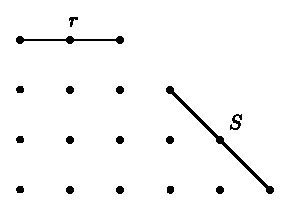
\includegraphics{vol2-figures/fig2.9.eps}}
  \end{figure}
  Take the uppermost row away and put it parallel to the last
  slope. This diminishes the number of rows by 1, so that a partition
  is switched over from the `even' class to the `odd' class or
  conversely. 
\end{enumerate}

Therefore there exists a one-one correspondence between the two
classes. So we have proved a theorem, which is a wrong one! because we
have not taken account of the exceptional case of pentagonal
numbers. The fallacy lies in having overlooked the fact that the last
slope may extend right up to the first row; the slope and the row may
very well interfere. Let us take one such instance. Let again $s< r$.
  \begin{figure}[H]
    \centering{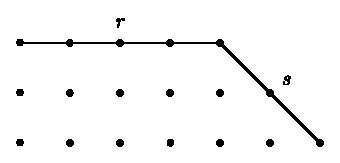
\includegraphics{vol2-figures/fig2.10.eps}}
  \end{figure}

If\pageoriginale  we place the last slope above the first row this works because the
number of points in the first row is also diminished by one, in fact
by the disputed point (notice again that no two rows are equal for $s<
r-1$). So the interference is of no account. With $s \geq r$ we may
again have an interfering case. We again place the top row
  \begin{figure}[H]
    \centering{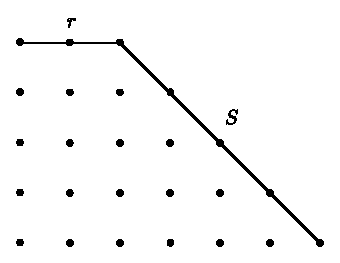
\includegraphics{vol2-figures/fig2.11.eps}}
  \end{figure}
\noindent behind the last slope, this time with a punishment. We have now
shortened the slope by 1. For $s-1\geq r$ the method is still good. So
the only cases of earnest interference are:

\begin{enumerate}[(i)]
\item $s<r$ but $x \geq r-1$. Then $r-1 \leq s \leq r$ and hence
  $s=r-1$
\item $s \geq r$ but $s- 1< r$. Then $s \geq r> s-1$ and hence $s=r$.
\end{enumerate}

Here we have something which can no longer be overcome. These are the
cases of pentagonal numbers. In (ii) the total number of dots is equal
to 
\begin{gather*}
  s+ (s+1) + (s+2) + \cdots + (2s-1)\\
  = \frac{s(3 s-1)}{2}
\end{gather*}
\begin{tabbing}
  In (i) this number \= $= (s+1)+ (s-2)+ \cdots + 2 s$\\
  \> $= \dfrac{s(3s+1)}{2}$
\end{tabbing}

These decompositions do not have companions. In general every
partition into one parity of different summands has a companion of the
other parity of different summands; and in the case of pentagonal
numbers there is just\pageoriginale  one in excess in one of the classes.

We now come to the most important application of identity
(\ref{part1:lec4:eq1}). Since 
$$
\frac{1}{\prod^\infty_{m=1} (1-x^m)}= \sum^\infty_{n=0} p(n) x^n,
$$ 
we have on combining this with (\ref{part1:lec4:eq1}),
\begin{equation*}
  1= \sum^\infty_{n=0} p(n) x^n \sum^\infty_{\lambda=-\infty}
  (-)^\lambda x^{\lambda (3 \lambda -1)/2} \tag{2}\label{part1:lec4:eq2}
\end{equation*}
This tells us the following story. All the coefficients on the right
side of (\ref{part1:lec4:eq2}) excepting the first must be zero. The typical exponent in
the second factor on the right side is $\lambda (3 \lambda-1)/2=
\omega_\lambda$, say. (The first few $\omega'_\lambda s$ are 0, 1, 2, 5,
 7, 12, 15, $\ldots$). Now look for $x^n$. Since the coefficient in
the first factor is $p(n)$ and that in the second always $\pm 1$, we
have, since $x^n (n \neq 0)$ does not appear on the left side
\begin{equation*}
  p(n) - p(n-1)- p(n-2)+ p(n-5) + p(n-7) -- ++ \cdots
  =0
\end{equation*}
or 

\begin{equation*}
  \sum_{0 \leq \omega_\lambda \leq n} p(n-
  \omega_\lambda) (-)^\lambda= 0 \tag{3}\label{part1:lec4:eq3}
\end{equation*}

This is a formula of recursion. Omitting the first index of summation
(\ref{part1:lec4:eq3}) gives
\begin{equation*}
  p(n) = \sum_{0 < \omega_\lambda \leq n} (-)^{\lambda-1}
  p(n-\omega_\lambda) \tag{4}\label{part1:lec4:eq4}
\end{equation*}

Let us calculate the first few $p(n)$.

\begin{align*}
  p(0) & = 1\\
  p(1) & = p(1-1)= p(0)=1\\
  p(2) & = p(2-1) + p(2-2)=2\\
  p(3) & = p(3-1)+ p(3-2)=3\\
  p(4) & = p(4-1)+ p(4-2)=5\\
  p(5) & = p(5-1)+ p(5-2)-p(5-5)=7\\
\end{align*}
(Watch!\pageoriginale  a pentagonal number - and a negative sign comes into
action!). These formulae get longer and longer, but not excessively
so. Let us estimate how long these will be. Since $\omega_\lambda \leq
n$ we have to look for $\lambda$ satisfying $\dfrac{\lambda(3 \lambda
  -1)}{2} \leq n$, which gives
\begin{align*}
  12 \lambda (3 \lambda -1) & \leq 24 n,\\
  36 \lambda^2 -12\lambda  & \leq 24 n,\\  
  (5 \lambda -1)^2 & = 24 n+1,\\
  |6 \lambda -1 | & = \sqrt{24n+1},\\
  |\lambda - \frac{1}{6}| & \leq \frac{1}{6} \sqrt{24n+1}.
\end{align*}

Hence roughly there will be $\dfrac{1}{3} \sqrt{24n} =
\dfrac{2}{3}\sqrt{6n}$ summands on the left side of (\ref{part1:lec4:eq3}). So their
number increases with the square root of $n$- the expressions do not
get too long after all (for $n=100$, we have 17 terms).

These formulae have been used for preparing tables of $p(n)$ which
have been quite useful. For instance Ramanujan discovered some of the
divisibility properties of $p(n)$ by using them. In the famous paper\pageoriginale 
of Hardy and Ramanujan (1917) there is a table of $p(n)$ for $n \leq
200$. These were computed by Macmahon, by using the above formulae and
the values were checked with those given by the Hardy-Ramanujan
formula. The asymptotic values were found to be very close to what
Macmahon computed. Gupta has extended the table for $p(n)$ up to 600. 

Before making another application of Euler's pentagonal theorem, we
proceed a bit further into the theory of formal power series. We add
now one more formal procedure, that of formal differentiation. Let 
$$
A =a_\circ + a_1 x+ a_2 x^2 + \cdots
$$

The derivative $A'$ of $A$ is by definition
$$
A' = a_1 + 2a_2 x + 3 a_3 x^2+ \cdots
$$

This is again a power series in our sense. This operation of
differentiation which produces one power series from another is a
linear operation:
$$
(A+B)' = A' + B',
$$
where $B$ is a second power series. This is easy to verify; actually
we need do this only for polynomials as everything is true modulo
$x^N$. Again,
$$
(c\, A)' = c \,A'
$$
as can be seen directly. Also
$$
(A \cdot B)' = A' B+ A \,B'.
$$

Let us look into this situation. Start with the simplest case, $A=
x^m$, $B= x^n$. Then 
\begin{align*}
  A' & = mx^{m-1}, \qquad B' = nx^{n-1} \\
  \text{and} \hspace{2.7cm} (AB)'  & = (x^{m+n})'=
  (m+n)x^{m+n-1},\hspace{3cm}\\  
  \text{also} \hspace{2cm} A'B+ AB' &=mx^{m-1+n} + nx^{m+n-1}\\
  & = (m+n)x^{m+n-1}
\end{align*}

So\pageoriginale  this is true also for polynomials by linearity, we can do it
piecemeal. And as it is enough if we stop short at $x^N$, it is true
in general,

Let us add one more remark. Let us write down a special case where $A$
and $B$ have reciprocals. Then $AB$ has a reciprocal too (since the
units form a group). In this case we have
$$
\frac{(AB)'}{AB} = \frac{A'}{A} + \frac{B'}{B},
$$
which is the rule for logarithmic differentiation. (It is identical
with the procedure in the calculus, as soon as we speak of
functions). For $A$, $B$ and $C$,
$$
\displaylines{\hfill 
  (ABC)' = A'(BC) + A(BC)' = A'BC+ AB'C+ABC'\hfill \cr
\text{or} \hfill \frac{(ABC)'}{ABC} = \frac{A'}{A} + \frac{B'}{B} +
\frac{C'}{C}, \hfill }
$$
and so on; in general, 
$$
\frac{\left( \prod^K_{n=1} A_k\right)'}{\prod^K_{k=1} A_k} =
\sum^K_{k=1} \frac{A'K}{A_k}
$$

We can do this for infinite products also if the products are
permissible. Indeed $\prod\limits^K_{k=1} A_k$ is legitimate if
$A_\ell = 1+ a_{\ell (k)} x^\ell + \cdots$ Consider modulo $x^N$;
break at a finite spot and the factors 1 will come into action. 


